\documentclass[a4paper]{article}

%% Language and font encodings
\usepackage[english]{babel}
\usepackage[utf8x]{inputenc}
\usepackage[T1]{fontenc}

%% Sets page size and margins
\usepackage[a4paper,top=3cm,bottom=2cm,left=3cm,right=3cm,marginparwidth=1.75cm]{geometry}

%% Useful packages
\usepackage{amsmath}
\usepackage{graphicx}
\usepackage[colorinlistoftodos]{todonotes}
\usepackage[colorlinks=true, allcolors=blue]{hyperref}

\title{Documentation de conception}
\author{\'Equipe GL 58}

\begin{document}
\maketitle

\section{Partie A}

\subsection{Les classes supplémentaires par rapport à la documentation actuelle}

Le schéma en page suivante représente l'arbre de relation des différentes classes du package tree de ce projet.\\ Les relations d'extension sont représentés par des liens, avec, quand le sens de la relation d'extension est ambigu, un rectangle au bout du lien, du côté de la superclasse. Ainsi, AbstractIdentifier étend AbstractLValue. \\

En bleu sont représentés les classes qui existaient déjà partiellement dans la notice précédente. En jaune sont les classes que nous avons récemment créées.\\
\begin{itemize}
\item AbstractDeclMethod,DeclMethod,AbstractDeclParam,DeclParam,AbstractDeclField,DeclField, ont dû être créées pour implémenter le concept de classe.\\
Ces derniers héritent de leur abstract associés dans 3 des cas, ou de Tree directement dans le cas des abstracts. Les règles les concernant sont déjà décrites dans la documentation précédente.\\

\item ListDeclMethod,ListDeclParam et ListDeclField ont été par conséquent créées, pour conserver une certaine homogénéité dans l'organisation de l'arbre et de l'analyseur syntaxique.\\
Ils héritent donc de TreeList.\\
Une astuce de code similaire à celle utilisée pour ListDeclVar a été utilisée pour ListDeclField, c'est-à-dire utiliser du passage de paramètre descendant vers la règle decl\_field, pour fournir les paramètres de visibilité et la liste à remplir.\\

\item L'implémentation des méthodes a nécessité de créer le noeud-classe Return.\\

\item This, Null, New et InstanceOf ont été créés comme conséquence de l'apparition du concept de classe.\\

\item L'accès aux paramètres et les appels aux méthodes ont une construction particulière :\\
CallMethod est un noeud représentant un appel à une méthode indépendamment de ce qui le précède, c'est-à-dire qu'il existe que ce soit pour un appel dans une méthode d'une classe qui appelle une autre des méthodes de cette classe (ou superclasse), ou un appel de méthodes spécifiant l'instance de classe à laquelle il est appliqué.\\
Dans le second cas, l'appel x.f(?) est représenté par une construction DotMethod ayant pour attribut un noeud CallMethod.\\
Le noeud Dot sert à accéder aux paramètres et hérite d'AbstractLValue.\\

\end{itemize}

\begin{figure}
\centering
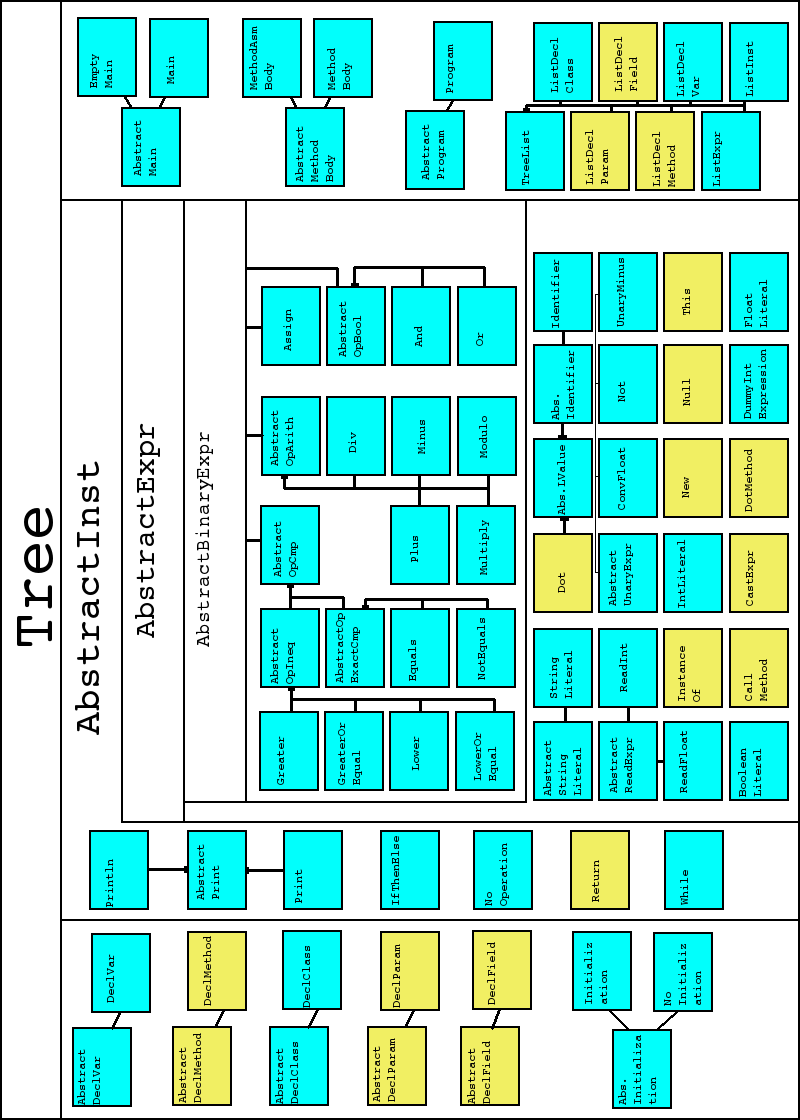
\includegraphics[width=1\textwidth]{SchemaTourne.png}
\caption{\label{fig:frog}Organisation du package tree.}
\end{figure}

\subsection{Information utile : la gestion des strings}
Le lexème STRING, en sortie d'analyseur, contient les guillemets au début et à la fin de la string, qui ont servis à l'identifier.\\
Ce problème est géré dans le parser, lors de l'analyse de StringLiteral, à l'aide de la ligne :\\
\texttt{\$tree=new StringLiteral( \$str.text.substring(1,\$str.text.length()-1) );}

\end{document}
